\documentclass[1p]{elsarticle_modified}
%\bibliographystyle{elsarticle-num}

%\usepackage[colorlinks]{hyperref}
%\usepackage{abbrmath_seonhwa} %\Abb, \Ascr, \Acal ,\Abf, \Afrak
\usepackage{amsfonts}
\usepackage{amssymb}
\usepackage{amsmath}
\usepackage{amsthm}
\usepackage{scalefnt}
\usepackage{amsbsy}
\usepackage{kotex}
\usepackage{caption}
\usepackage{subfig}
\usepackage{color}
\usepackage{graphicx}
\usepackage{xcolor} %% white, black, red, green, blue, cyan, magenta, yellow
\usepackage{float}
\usepackage{setspace}
\usepackage{hyperref}

\usepackage{tikz}
\usetikzlibrary{arrows}

\usepackage{multirow}
\usepackage{array} % fixed length table
\usepackage{hhline}

%%%%%%%%%%%%%%%%%%%%%
\makeatletter
\renewcommand*\env@matrix[1][\arraystretch]{%
	\edef\arraystretch{#1}%
	\hskip -\arraycolsep
	\let\@ifnextchar\new@ifnextchar
	\array{*\c@MaxMatrixCols c}}
\makeatother %https://tex.stackexchange.com/questions/14071/how-can-i-increase-the-line-spacing-in-a-matrix
%%%%%%%%%%%%%%%

\usepackage[normalem]{ulem}

\newcommand{\msout}[1]{\ifmmode\text{\sout{\ensuremath{#1}}}\else\sout{#1}\fi}
%SOURCE: \msout is \stkout macro in https://tex.stackexchange.com/questions/20609/strikeout-in-math-mode

\newcommand{\cancel}[1]{
	\ifmmode
	{\color{red}\msout{#1}}
	\else
	{\color{red}\sout{#1}}
	\fi
}

\newcommand{\add}[1]{
	{\color{blue}\uwave{#1}}
}

\newcommand{\replace}[2]{
	\ifmmode
	{\color{red}\msout{#1}}{\color{blue}\uwave{#2}}
	\else
	{\color{red}\sout{#1}}{\color{blue}\uwave{#2}}
	\fi
}

\newcommand{\Sol}{\mathcal{S}} %segment
\newcommand{\D}{D} %diagram
\newcommand{\A}{\mathcal{A}} %arc


%%%%%%%%%%%%%%%%%%%%%%%%%%%%%5 test

\def\sl{\operatorname{\textup{SL}}(2,\Cbb)}
\def\psl{\operatorname{\textup{PSL}}(2,\Cbb)}
\def\quan{\mkern 1mu \triangleright \mkern 1mu}

\theoremstyle{definition}
\newtheorem{thm}{Theorem}[section]
\newtheorem{prop}[thm]{Proposition}
\newtheorem{lem}[thm]{Lemma}
\newtheorem{ques}[thm]{Question}
\newtheorem{cor}[thm]{Corollary}
\newtheorem{defn}[thm]{Definition}
\newtheorem{exam}[thm]{Example}
\newtheorem{rmk}[thm]{Remark}
\newtheorem{alg}[thm]{Algorithm}

\newcommand{\I}{\sqrt{-1}}
\begin{document}

%\begin{frontmatter}
%
%\title{Boundary parabolic representations of knots up to 8 crossings}
%
%%% Group authors per affiliation:
%\author{Yunhi Cho} 
%\address{Department of Mathematics, University of Seoul, Seoul, Korea}
%\ead{yhcho@uos.ac.kr}
%
%
%\author{Seonhwa Kim} %\fnref{s_kim}}
%\address{Center for Geometry and Physics, Institute for Basic Science, Pohang, 37673, Korea}
%\ead{ryeona17@ibs.re.kr}
%
%\author{Hyuk Kim}
%\address{Department of Mathematical Sciences, Seoul National University, Seoul 08826, Korea}
%\ead{hyukkim@snu.ac.kr}
%
%\author{Seokbeom Yoon}
%\address{Department of Mathematical Sciences, Seoul National University, Seoul, 08826,  Korea}
%\ead{sbyoon15@snu.ac.kr}
%
%\begin{abstract}
%We find all boundary parabolic representation of knots up to 8 crossings.
%
%\end{abstract}
%\begin{keyword}
%    \MSC[2010] 57M25 
%\end{keyword}
%
%\end{frontmatter}

%\linenumbers
%\tableofcontents
%
\newcommand\colored[1]{\textcolor{white}{\rule[-0.35ex]{0.8em}{1.4ex}}\kern-0.8em\color{red} #1}%
%\newcommand\colored[1]{\textcolor{white}{ #1}\kern-2.17ex	\textcolor{white}{ #1}\kern-1.81ex	\textcolor{white}{ #1}\kern-2.15ex\color{red}#1	}

{\Large $\underline{10_{122}~(K10a_{89})}$}

\setlength{\tabcolsep}{10pt}
\renewcommand{\arraystretch}{1.6}
\vspace{1cm}\begin{tabular}{m{100pt}>{\centering\arraybackslash}m{274pt}}
\multirow{5}{120pt}{
	\centering
	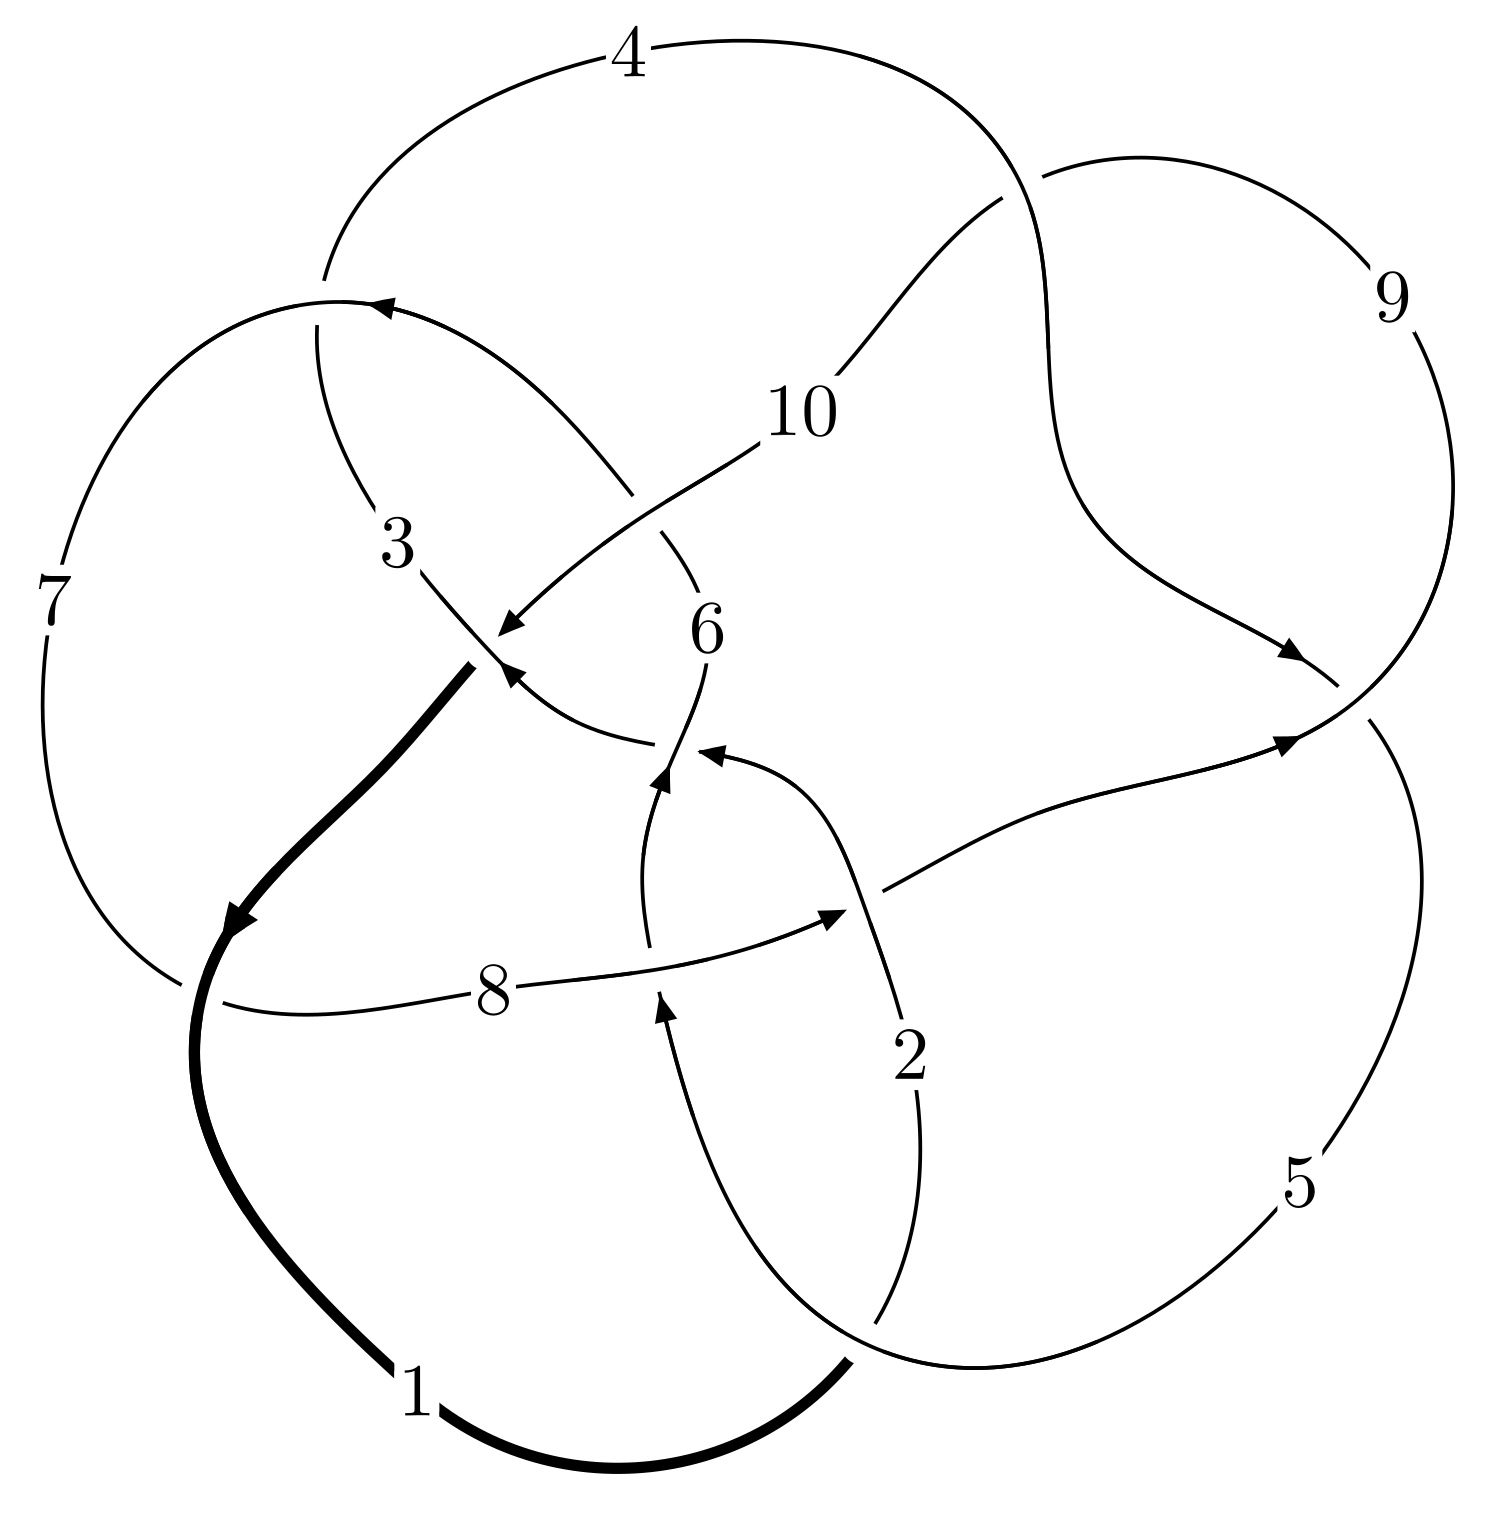
\includegraphics[width=112pt]{../../../GIT/diagram.site/Diagrams/png/206_10_122.png}\\
\ \ \ A knot diagram\footnotemark}&
\allowdisplaybreaks
\textbf{Linearized knot diagam} \\
\cline{2-2}
 &
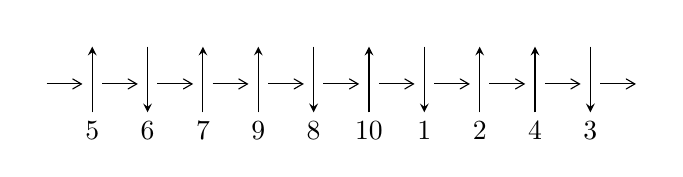
\begin{tikzpicture}[x=20pt, y=17pt]
	% nodes
	\node (C0) at (0, 0) {};
	\node (C1) at (1, 0) {};
	\node (C1U) at (1, +1) {};
	\node (C1D) at (1, -1) {5};

	\node (C2) at (2, 0) {};
	\node (C2U) at (2, +1) {};
	\node (C2D) at (2, -1) {6};

	\node (C3) at (3, 0) {};
	\node (C3U) at (3, +1) {};
	\node (C3D) at (3, -1) {7};

	\node (C4) at (4, 0) {};
	\node (C4U) at (4, +1) {};
	\node (C4D) at (4, -1) {9};

	\node (C5) at (5, 0) {};
	\node (C5U) at (5, +1) {};
	\node (C5D) at (5, -1) {8};

	\node (C6) at (6, 0) {};
	\node (C6U) at (6, +1) {};
	\node (C6D) at (6, -1) {10};

	\node (C7) at (7, 0) {};
	\node (C7U) at (7, +1) {};
	\node (C7D) at (7, -1) {1};

	\node (C8) at (8, 0) {};
	\node (C8U) at (8, +1) {};
	\node (C8D) at (8, -1) {2};

	\node (C9) at (9, 0) {};
	\node (C9U) at (9, +1) {};
	\node (C9D) at (9, -1) {4};

	\node (C10) at (10, 0) {};
	\node (C10U) at (10, +1) {};
	\node (C10D) at (10, -1) {3};
	\node (C11) at (11, 0) {};

	% arrows
	\draw[->,>={angle 60}]
	(C0) edge (C1) (C1) edge (C2) (C2) edge (C3) (C3) edge (C4) (C4) edge (C5) (C5) edge (C6) (C6) edge (C7) (C7) edge (C8) (C8) edge (C9) (C9) edge (C10) (C10) edge (C11) ;	\draw[->,>=stealth]
	(C1D) edge (C1U) (C2U) edge (C2D) (C3D) edge (C3U) (C4D) edge (C4U) (C5U) edge (C5D) (C6D) edge (C6U) (C7U) edge (C7D) (C8D) edge (C8U) (C9D) edge (C9U) (C10U) edge (C10D) ;
	\end{tikzpicture} \\
\hhline{~~} \\& 
\textbf{Solving Sequence} \\ \cline{2-2} 
 &
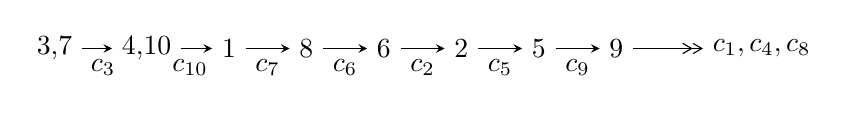
\begin{tikzpicture}[x=28pt, y=7pt]
	% node
	\node (A0) at (-1/8, 0) {3,7};
	\node (A1) at (17/16, 0) {4,10};
	\node (A2) at (17/8, 0) {1};
	\node (A3) at (25/8, 0) {8};
	\node (A4) at (33/8, 0) {6};
	\node (A5) at (41/8, 0) {2};
	\node (A6) at (49/8, 0) {5};
	\node (A7) at (57/8, 0) {9};
	\node (C1) at (1/2, -1) {$c_{3}$};
	\node (C2) at (13/8, -1) {$c_{10}$};
	\node (C3) at (21/8, -1) {$c_{7}$};
	\node (C4) at (29/8, -1) {$c_{6}$};
	\node (C5) at (37/8, -1) {$c_{2}$};
	\node (C6) at (45/8, -1) {$c_{5}$};
	\node (C7) at (53/8, -1) {$c_{9}$};
	\node (A8) at (9, 0) {$c_{1},c_{4},c_{8}$};

	% edge
	\draw[->,>=stealth]	
	(A0) edge (A1) (A1) edge (A2) (A2) edge (A3) (A3) edge (A4) (A4) edge (A5) (A5) edge (A6) (A6) edge (A7) ;
	\draw[->>,>={angle 60}]	
	(A7) edge (A8);
\end{tikzpicture} \\ 

\end{tabular} \\

\footnotetext{
The image of knot diagram is generated by the software ``\textbf{Draw programme}" developed by Andrew Bartholomew(\url{http://www.layer8.co.uk/maths/draw/index.htm\#Running-draw}), where we modified some parts for our purpose(\url{https://github.com/CATsTAILs/LinksPainter}).
}\phantom \\ \newline 
\centering \textbf{Ideals for irreducible components\footnotemark of $X_{\text{par}}$} 
 
\begin{align*}
I^u_{1}&=\langle 
- u^4- u^3-4 u^2+6 b+u+3,\;a+1,\;u^5+u^4+u^3- u^2+3 u+3\rangle \\
I^u_{2}&=\langle 
u^9-3 u^8+2 u^7- u^6- u^5-8 u^4+u^3-5 u^2+4 b- u+3,\;a+1,\;u^{10}+u^8+u^7+4 u^6+u^5+u^4-2 u^3+1\rangle \\
I^u_{3}&=\langle 
1.44071\times10^{22} u^{23}+2.00575\times10^{22} u^{22}+\cdots+8.55063\times10^{22} b+4.63180\times10^{23},\\
\phantom{I^u_{3}}&\phantom{= \langle  }6.78118\times10^{27} u^{23}+1.02960\times10^{28} u^{22}+\cdots+1.85674\times10^{28} a+3.22471\times10^{29},\;u^{24}+u^{23}+\cdots-26 u+67\rangle \\
I^u_{4}&=\langle 
118 u^{11}-136 u^{10}+\cdots+209 b-456,\;-142 u^{11}-116 u^{10}+\cdots+209 a-90,\\
\phantom{I^u_{4}}&\phantom{= \langle  }u^{12}- u^{11}+2 u^{10}+u^9+2 u^8-9 u^7+3 u^6+3 u^5+2 u^4-8 u^3+8 u^2-4 u+1\rangle \\
I^u_{5}&=\langle 
u^5+2 u^4-4 u^3+u^2+12 b+5 u+3,\;a+1,\;u^6- u^5+2 u^4+u^3+2 u^2+3\rangle \\
I^u_{6}&=\langle 
b+u+1,\;a+1,\;u^2+u+1\rangle \\
I^u_{7}&=\langle 
b-1,\;-3 u^5-4 u^4-6 u^3+6 u^2+a-7 u+1,\;u^6+u^5+2 u^4-2 u^3+4 u^2-2 u+1\rangle \\
I^u_{8}&=\langle 
b,\;a+1,\;u^3- u^2+1\rangle \\
\\
\end{align*}
\raggedright * 8 irreducible components of $\dim_{\mathbb{C}}=0$, with total 68 representations.\\
\footnotetext{All coefficients of polynomials are rational numbers. But the coefficients are sometimes approximated in decimal forms when there is not enough margin.}
\newpage
\renewcommand{\arraystretch}{1}
\centering \section*{I. $I^u_{1}= \langle - u^4- u^3-4 u^2+6 b+u+3,\;a+1,\;u^5+u^4+u^3- u^2+3 u+3 \rangle$}
\flushleft \textbf{(i) Arc colorings}\\
\begin{tabular}{m{7pt} m{180pt} m{7pt} m{180pt} }
\flushright $a_{3}=$&$\begin{pmatrix}1\\0\end{pmatrix}$ \\
\flushright $a_{7}=$&$\begin{pmatrix}0\\u\end{pmatrix}$ \\
\flushright $a_{4}=$&$\begin{pmatrix}1\\- u^2\end{pmatrix}$ \\
\flushright $a_{10}=$&$\begin{pmatrix}-1\\\frac{1}{6} u^4+\frac{1}{6} u^3+\cdots-\frac{1}{6} u-\frac{1}{2}\end{pmatrix}$ \\
\flushright $a_{1}=$&$\begin{pmatrix}-\frac{1}{6} u^4-\frac{1}{6} u^3+\cdots+\frac{1}{6} u-\frac{1}{2}\\\frac{1}{6} u^4+\frac{1}{6} u^3+\cdots-\frac{1}{6} u-\frac{1}{2}\end{pmatrix}$ \\
\flushright $a_{8}=$&$\begin{pmatrix}\frac{1}{3} u^4+\frac{1}{3} u^3+\frac{1}{3} u^2+\frac{2}{3} u+1\\-\frac{1}{3} u^4-\frac{5}{6} u^3+\cdots+\frac{1}{3} u-\frac{1}{2}\end{pmatrix}$ \\
\flushright $a_{6}=$&$\begin{pmatrix}- u\\\frac{1}{2} u^3-\frac{1}{2}\end{pmatrix}$ \\
\flushright $a_{2}=$&$\begin{pmatrix}\frac{1}{2} u^4-\frac{1}{2} u+1\\u^2-1\end{pmatrix}$ \\
\flushright $a_{5}=$&$\begin{pmatrix}\frac{1}{6} u^4-\frac{1}{6} u^3+\cdots+\frac{1}{2} u+\frac{5}{6}\\-\frac{1}{2} u^4-\frac{2}{3} u^3+\cdots-\frac{7}{6} u-\frac{4}{3}\end{pmatrix}$ \\
\flushright $a_{9}=$&$\begin{pmatrix}-\frac{1}{6} u^4-\frac{1}{6} u^3+\cdots+\frac{1}{6} u-\frac{1}{2}\\-\frac{1}{3} u^4+\frac{1}{6} u^3+\cdots-\frac{2}{3} u-\frac{1}{2}\end{pmatrix}$\\&\end{tabular}
\flushleft \textbf{(ii) Obstruction class $= -1$}\\~\\
\flushleft \textbf{(iii) Cusp Shapes $= \frac{17}{9} u^4-\frac{7}{9} u^3-\frac{28}{9} u^2-\frac{35}{9} u+7$}\\~\\
\newpage\renewcommand{\arraystretch}{1}
\flushleft \textbf{(iv) u-Polynomials at the component}\newline \\
\begin{tabular}{m{50pt}|m{274pt}}
Crossings & \hspace{64pt}u-Polynomials at each crossing \\
\hline $$\begin{aligned}c_{1},c_{3},c_{6}\\c_{8}\end{aligned}$$&$\begin{aligned}
&u^5- u^4+u^3+u^2+3 u-3
\end{aligned}$\\
\hline $$\begin{aligned}c_{2},c_{7}\end{aligned}$$&$\begin{aligned}
&u^5-3 u^3+7 u-4
\end{aligned}$\\
\hline $$\begin{aligned}c_{4},c_{9}\end{aligned}$$&$\begin{aligned}
&3(3 u^5-12 u^4+26 u^3-36 u^2+28 u-8)
\end{aligned}$\\
\hline $$\begin{aligned}c_{5},c_{10}\end{aligned}$$&$\begin{aligned}
&3(3 u^5-15 u^4+35 u^3-41 u^2+23 u-1)
\end{aligned}$\\
\hline
\end{tabular}\\~\\
\newpage\renewcommand{\arraystretch}{1}
\flushleft \textbf{(v) Riley Polynomials at the component}\newline \\
\begin{tabular}{m{50pt}|m{274pt}}
Crossings & \hspace{64pt}Riley Polynomials at each crossing \\
\hline $$\begin{aligned}c_{1},c_{3},c_{6}\\c_{8}\end{aligned}$$&$\begin{aligned}
&y^5+y^4+9 y^3- y^2+15 y-9
\end{aligned}$\\
\hline $$\begin{aligned}c_{2},c_{7}\end{aligned}$$&$\begin{aligned}
&y^5-6 y^4+23 y^3-42 y^2+49 y-16
\end{aligned}$\\
\hline $$\begin{aligned}c_{4},c_{9}\end{aligned}$$&$\begin{aligned}
&9(9 y^5+12 y^4-20 y^3-32 y^2+208 y-64)
\end{aligned}$\\
\hline $$\begin{aligned}c_{5},c_{10}\end{aligned}$$&$\begin{aligned}
&9(9 y^5-15 y^4+133 y^3-101 y^2+447 y-1)
\end{aligned}$\\
\hline
\end{tabular}\\~\\
\newpage\flushleft \textbf{(vi) Complex Volumes and Cusp Shapes}
$$\begin{array}{c|c|c}  
\text{Solutions to }I^u_{1}& \I (\text{vol} + \sqrt{-1}CS) & \text{Cusp shape}\\
 \hline 
\begin{aligned}
u &= \phantom{-}0.860145 + 0.891716 I \\
a &= -1.00000\phantom{ +0.000000I} \\
b &= -1.30783 + 1.05747 I\end{aligned}
 & -1.64634 + 10.42060 I & \phantom{-}0.48885 - 9.54868 I \\ \hline\begin{aligned}
u &= \phantom{-}0.860145 - 0.891716 I \\
a &= -1.00000\phantom{ +0.000000I} \\
b &= -1.30783 - 1.05747 I\end{aligned}
 & -1.64634 - 10.42060 I & \phantom{-}0.48885 + 9.54868 I \\ \hline\begin{aligned}
u &= -0.724026\phantom{ +0.000000I} \\
a &= -1.00000\phantom{ +0.000000I} \\
b &= -0.0473103\phantom{ +0.000000I}\end{aligned}
 & \phantom{-}1.11365\phantom{ +0.000000I} & \phantom{-}8.99900\phantom{ +0.000000I} \\ \hline\begin{aligned}
u &= -0.99813 + 1.30502 I \\
a &= -1.00000\phantom{ +0.000000I} \\
b &= -1.16851 - 1.06085 I\end{aligned}
 & -7.9576 - 16.4108 I & -1.98837 + 8.68093 I \\ \hline\begin{aligned}
u &= -0.99813 - 1.30502 I \\
a &= -1.00000\phantom{ +0.000000I} \\
b &= -1.16851 + 1.06085 I\end{aligned}
 & -7.9576 + 16.4108 I & -1.98837 - 8.68093 I\\
 \hline 
 \end{array}$$\newpage\newpage\renewcommand{\arraystretch}{1}
\centering \section*{II. $I^u_{2}= \langle u^9-3 u^8+\cdots+4 b+3,\;a+1,\;u^{10}+u^8+u^7+4 u^6+u^5+u^4-2 u^3+1 \rangle$}
\flushleft \textbf{(i) Arc colorings}\\
\begin{tabular}{m{7pt} m{180pt} m{7pt} m{180pt} }
\flushright $a_{3}=$&$\begin{pmatrix}1\\0\end{pmatrix}$ \\
\flushright $a_{7}=$&$\begin{pmatrix}0\\u\end{pmatrix}$ \\
\flushright $a_{4}=$&$\begin{pmatrix}1\\- u^2\end{pmatrix}$ \\
\flushright $a_{10}=$&$\begin{pmatrix}-1\\-\frac{1}{4} u^9+\frac{3}{4} u^8+\cdots+\frac{1}{4} u-\frac{3}{4}\end{pmatrix}$ \\
\flushright $a_{1}=$&$\begin{pmatrix}\frac{1}{4} u^9-\frac{3}{4} u^8+\cdots-\frac{1}{4} u-\frac{1}{4}\\-\frac{1}{4} u^9+\frac{3}{4} u^8+\cdots+\frac{1}{4} u-\frac{3}{4}\end{pmatrix}$ \\
\flushright $a_{8}=$&$\begin{pmatrix}\frac{3}{4} u^9-\frac{3}{4} u^8+\cdots+\frac{5}{4} u+\frac{3}{4}\\-\frac{3}{2} u^9+u^8+\cdots-\frac{1}{2} u-1\end{pmatrix}$ \\
\flushright $a_{6}=$&$\begin{pmatrix}- u\\\frac{3}{4} u^9-\frac{1}{4} u^8+\cdots+\frac{1}{4} u+\frac{1}{4}\end{pmatrix}$ \\
\flushright $a_{2}=$&$\begin{pmatrix}-\frac{1}{4} u^9-\frac{1}{4} u^8+\cdots+\frac{1}{4} u+\frac{1}{4}\\-\frac{3}{4} u^9-\frac{1}{4} u^8+\cdots+\frac{3}{4} u-\frac{3}{4}\end{pmatrix}$ \\
\flushright $a_{5}=$&$\begin{pmatrix}\frac{3}{2} u^9- u^8+\cdots+\frac{1}{2} u+1\\-\frac{5}{4} u^9+\frac{3}{4} u^8+\cdots+\frac{5}{4} u-\frac{7}{4}\end{pmatrix}$ \\
\flushright $a_{9}=$&$\begin{pmatrix}\frac{1}{4} u^9-\frac{3}{4} u^8+\cdots-\frac{1}{4} u-\frac{1}{4}\\-\frac{1}{2} u^9+\frac{1}{2} u^8+\cdots+\frac{1}{2} u-\frac{3}{2}\end{pmatrix}$\\&\end{tabular}
\flushleft \textbf{(ii) Obstruction class $= -1$}\\~\\
\flushleft \textbf{(iii) Cusp Shapes $= -\frac{1}{4} u^9+\frac{5}{4} u^8-\frac{5}{2} u^7+\frac{5}{4} u^6+\frac{11}{4} u^5-\frac{9}{4} u^3+\frac{15}{4} u^2+\frac{25}{4} u+\frac{7}{4}$}\\~\\
\newpage\renewcommand{\arraystretch}{1}
\flushleft \textbf{(iv) u-Polynomials at the component}\newline \\
\begin{tabular}{m{50pt}|m{274pt}}
Crossings & \hspace{64pt}u-Polynomials at each crossing \\
\hline $$\begin{aligned}c_{1},c_{3},c_{6}\\c_{8}\end{aligned}$$&$\begin{aligned}
&u^{10}+u^8- u^7+4 u^6- u^5+u^4+2 u^3+1
\end{aligned}$\\
\hline $$\begin{aligned}c_{2},c_{7}\end{aligned}$$&$\begin{aligned}
&(u^5- u^4+1)^2
\end{aligned}$\\
\hline $$\begin{aligned}c_{4},c_{9}\end{aligned}$$&$\begin{aligned}
&(u^5-4 u^4+9 u^3-13 u^2+10 u-4)^2
\end{aligned}$\\
\hline $$\begin{aligned}c_{5},c_{10}\end{aligned}$$&$\begin{aligned}
&u^{10}-10 u^9+\cdots-95 u+19
\end{aligned}$\\
\hline
\end{tabular}\\~\\
\newpage\renewcommand{\arraystretch}{1}
\flushleft \textbf{(v) Riley Polynomials at the component}\newline \\
\begin{tabular}{m{50pt}|m{274pt}}
Crossings & \hspace{64pt}Riley Polynomials at each crossing \\
\hline $$\begin{aligned}c_{1},c_{3},c_{6}\\c_{8}\end{aligned}$$&$\begin{aligned}
&y^{10}+2 y^9+9 y^8+9 y^7+16 y^6+13 y^5+7 y^4+4 y^3+2 y^2+1
\end{aligned}$\\
\hline $$\begin{aligned}c_{2},c_{7}\end{aligned}$$&$\begin{aligned}
&(y^5- y^4+2 y^2-1)^2
\end{aligned}$\\
\hline $$\begin{aligned}c_{4},c_{9}\end{aligned}$$&$\begin{aligned}
&(y^5+2 y^4-3 y^3-21 y^2-4 y-16)^2
\end{aligned}$\\
\hline $$\begin{aligned}c_{5},c_{10}\end{aligned}$$&$\begin{aligned}
&y^{10}-4 y^9+\cdots+361 y+361
\end{aligned}$\\
\hline
\end{tabular}\\~\\
\newpage\flushleft \textbf{(vi) Complex Volumes and Cusp Shapes}
$$\begin{array}{c|c|c}  
\text{Solutions to }I^u_{2}& \I (\text{vol} + \sqrt{-1}CS) & \text{Cusp shape}\\
 \hline 
\begin{aligned}
u &= -0.186488 + 0.884166 I \\
a &= -1.00000\phantom{ +0.000000I} \\
b &= -1.29181 + 1.28122 I\end{aligned}
 & -7.58413 - 7.68015 I & -6.00758 + 6.55636 I \\ \hline\begin{aligned}
u &= -0.186488 - 0.884166 I \\
a &= -1.00000\phantom{ +0.000000I} \\
b &= -1.29181 - 1.28122 I\end{aligned}
 & -7.58413 + 7.68015 I & -6.00758 - 6.55636 I \\ \hline\begin{aligned}
u &= -0.583652 + 0.627090 I \\
a &= -1.00000\phantom{ +0.000000I} \\
b &= -1.68130 - 0.73200 I\end{aligned}
 & -1.88219\phantom{ +0.000000I} &                  -6
-1.264578 + 0. 10   I\phantom{ +0.000000I} \\ \hline\begin{aligned}
u &= -0.583652 - 0.627090 I \\
a &= -1.00000\phantom{ +0.000000I} \\
b &= -1.68130 + 0.73200 I\end{aligned}
 & -1.88219\phantom{ +0.000000I} &                  -6
-1.264578 + 0. 10   I\phantom{ +0.000000I} \\ \hline\begin{aligned}
u &= -0.837561 + 0.788016 I \\
a &= -1.00000\phantom{ +0.000000I} \\
b &= -0.560268 - 0.657796 I\end{aligned}
 & \phantom{-}1.94548 - 2.30273 I & \phantom{-}6.63987 + 2.99878 I \\ \hline\begin{aligned}
u &= -0.837561 - 0.788016 I \\
a &= -1.00000\phantom{ +0.000000I} \\
b &= -0.560268 + 0.657796 I\end{aligned}
 & \phantom{-}1.94548 + 2.30273 I & \phantom{-}6.63987 - 2.99878 I \\ \hline\begin{aligned}
u &= \phantom{-}0.656329 + 0.295939 I \\
a &= -1.00000\phantom{ +0.000000I} \\
b &= -0.297621 + 1.050690 I\end{aligned}
 & \phantom{-}1.94548 - 2.30273 I & \phantom{-}6.63987 + 2.99878 I \\ \hline\begin{aligned}
u &= \phantom{-}0.656329 - 0.295939 I \\
a &= -1.00000\phantom{ +0.000000I} \\
b &= -0.297621 - 1.050690 I\end{aligned}
 & \phantom{-}1.94548 + 2.30273 I & \phantom{-}6.63987 - 2.99878 I \\ \hline\begin{aligned}
u &= \phantom{-}0.95137 + 1.23664 I \\
a &= -1.00000\phantom{ +0.000000I} \\
b &= -1.169000 + 0.742016 I\end{aligned}
 & -7.58413 + 7.68015 I & -6.00758 - 6.55636 I \\ \hline\begin{aligned}
u &= \phantom{-}0.95137 - 1.23664 I \\
a &= -1.00000\phantom{ +0.000000I} \\
b &= -1.169000 - 0.742016 I\end{aligned}
 & -7.58413 - 7.68015 I & -6.00758 + 6.55636 I\\
 \hline 
 \end{array}$$\newpage\newpage\renewcommand{\arraystretch}{1}
\centering \section*{III. $I^u_{3}= \langle 1.44\times10^{22} u^{23}+2.01\times10^{22} u^{22}+\cdots+8.55\times10^{22} b+4.63\times10^{23},\;6.78\times10^{27} u^{23}+1.03\times10^{28} u^{22}+\cdots+1.86\times10^{28} a+3.22\times10^{29},\;u^{24}+u^{23}+\cdots-26 u+67 \rangle$}
\flushleft \textbf{(i) Arc colorings}\\
\begin{tabular}{m{7pt} m{180pt} m{7pt} m{180pt} }
\flushright $a_{3}=$&$\begin{pmatrix}1\\0\end{pmatrix}$ \\
\flushright $a_{7}=$&$\begin{pmatrix}0\\u\end{pmatrix}$ \\
\flushright $a_{4}=$&$\begin{pmatrix}1\\- u^2\end{pmatrix}$ \\
\flushright $a_{10}=$&$\begin{pmatrix}-0.365219 u^{23}-0.554519 u^{22}+\cdots-56.6942 u-17.3675\\-0.168492 u^{23}-0.234573 u^{22}+\cdots-18.0977 u-5.41691\end{pmatrix}$ \\
\flushright $a_{1}=$&$\begin{pmatrix}-0.196727 u^{23}-0.319946 u^{22}+\cdots-38.5965 u-11.9506\\-0.168492 u^{23}-0.234573 u^{22}+\cdots-18.0977 u-5.41691\end{pmatrix}$ \\
\flushright $a_{8}=$&$\begin{pmatrix}0.378827 u^{23}+0.547263 u^{22}+\cdots+70.2497 u+31.8889\\0.0711438 u^{23}+0.0997089 u^{22}+\cdots+6.43136 u+6.60068\end{pmatrix}$ \\
\flushright $a_{6}=$&$\begin{pmatrix}0.413307 u^{23}+0.527233 u^{22}+\cdots+69.0401 u+33.4117\\-0.0366636 u^{23}-0.119739 u^{22}+\cdots-5.64098 u-5.07784\end{pmatrix}$ \\
\flushright $a_{2}=$&$\begin{pmatrix}-0.531591 u^{23}-1.06310 u^{22}+\cdots-46.4641 u-72.9977\\-0.0738408 u^{23}-0.0393684 u^{22}+\cdots-4.06916 u+5.13154\end{pmatrix}$ \\
\flushright $a_{5}=$&$\begin{pmatrix}0.163715 u^{23}+0.0132091 u^{22}+\cdots+44.8521 u-33.5831\\0.0580226 u^{23}-0.0407545 u^{22}+\cdots+14.5495 u-11.8038\end{pmatrix}$ \\
\flushright $a_{9}=$&$\begin{pmatrix}-0.318510 u^{23}-0.571602 u^{22}+\cdots-58.1444 u-24.6338\\-0.0998054 u^{23}-0.191253 u^{22}+\cdots-13.3096 u-9.69092\end{pmatrix}$\\&\end{tabular}
\flushleft \textbf{(ii) Obstruction class $= -1$}\\~\\
\flushleft \textbf{(iii) Cusp Shapes $= -\frac{49507502818400620336471888}{55425173492754441021594851} u^{23}-\frac{25666816923514324973679840}{55425173492754441021594851} u^{22}+\cdots-\frac{8454714591899753146209998108}{55425173492754441021594851} u+\frac{3209287438838954049727512794}{55425173492754441021594851}$}\\~\\
\newpage\renewcommand{\arraystretch}{1}
\flushleft \textbf{(iv) u-Polynomials at the component}\newline \\
\begin{tabular}{m{50pt}|m{274pt}}
Crossings & \hspace{64pt}u-Polynomials at each crossing \\
\hline $$\begin{aligned}c_{1},c_{3},c_{6}\\c_{8}\end{aligned}$$&$\begin{aligned}
&u^{24}- u^{23}+\cdots+26 u+67
\end{aligned}$\\
\hline $$\begin{aligned}c_{2},c_{7}\end{aligned}$$&$\begin{aligned}
&(u^{12}- u^{11}+\cdots-24 u+19)^{2}
\end{aligned}$\\
\hline $$\begin{aligned}c_{4},c_{9}\end{aligned}$$&$\begin{aligned}
&(u^3+u^2+2 u+1)^8
\end{aligned}$\\
\hline $$\begin{aligned}c_{5},c_{10}\end{aligned}$$&$\begin{aligned}
&(u^4+u^3-2 u+1)^6
\end{aligned}$\\
\hline
\end{tabular}\\~\\
\newpage\renewcommand{\arraystretch}{1}
\flushleft \textbf{(v) Riley Polynomials at the component}\newline \\
\begin{tabular}{m{50pt}|m{274pt}}
Crossings & \hspace{64pt}Riley Polynomials at each crossing \\
\hline $$\begin{aligned}c_{1},c_{3},c_{6}\\c_{8}\end{aligned}$$&$\begin{aligned}
&y^{24}+9 y^{23}+\cdots+68200 y+4489
\end{aligned}$\\
\hline $$\begin{aligned}c_{2},c_{7}\end{aligned}$$&$\begin{aligned}
&(y^{12}-13 y^{11}+\cdots-2096 y+361)^{2}
\end{aligned}$\\
\hline $$\begin{aligned}c_{4},c_{9}\end{aligned}$$&$\begin{aligned}
&(y^3+3 y^2+2 y-1)^8
\end{aligned}$\\
\hline $$\begin{aligned}c_{5},c_{10}\end{aligned}$$&$\begin{aligned}
&(y^4- y^3+6 y^2-4 y+1)^6
\end{aligned}$\\
\hline
\end{tabular}\\~\\
\newpage\flushleft \textbf{(vi) Complex Volumes and Cusp Shapes}
$$\begin{array}{c|c|c}  
\text{Solutions to }I^u_{3}& \I (\text{vol} + \sqrt{-1}CS) & \text{Cusp shape}\\
 \hline 
\begin{aligned}
u &= \phantom{-}0.690412 + 0.835611 I \\
a &= \phantom{-}0.969409 + 0.292352 I \\
b &= \phantom{-}1.12196 - 1.05376 I\end{aligned}
 & -2.17641 + 4.05977 I & -2.98049 - 6.92820 I \\ \hline\begin{aligned}
u &= \phantom{-}0.690412 - 0.835611 I \\
a &= \phantom{-}0.969409 - 0.292352 I \\
b &= \phantom{-}1.12196 + 1.05376 I\end{aligned}
 & -2.17641 - 4.05977 I & -2.98049 + 6.92820 I \\ \hline\begin{aligned}
u &= -0.611027 + 0.676812 I \\
a &= -0.37068 + 1.40297 I \\
b &= -0.621964 - 0.187730 I\end{aligned}
 & -2.17641 - 4.05977 I & -2.98049 + 6.92820 I \\ \hline\begin{aligned}
u &= -0.611027 - 0.676812 I \\
a &= -0.37068 - 1.40297 I \\
b &= -0.621964 + 0.187730 I\end{aligned}
 & -2.17641 + 4.05977 I & -2.98049 - 6.92820 I \\ \hline\begin{aligned}
u &= -0.424999 + 1.011890 I \\
a &= \phantom{-}0.945558 + 0.285159 I \\
b &= \phantom{-}1.12196 + 1.05376 I\end{aligned}
 & -2.17641 - 4.05977 I & -2.98049 + 6.92820 I \\ \hline\begin{aligned}
u &= -0.424999 - 1.011890 I \\
a &= \phantom{-}0.945558 - 0.285159 I \\
b &= \phantom{-}1.12196 - 1.05376 I\end{aligned}
 & -2.17641 + 4.05977 I & -2.98049 - 6.92820 I \\ \hline\begin{aligned}
u &= \phantom{-}0.211529 + 0.854823 I \\
a &= -1.85383 + 1.20187 I \\
b &= -0.621964 + 0.187730 I\end{aligned}
 & -6.31400 + 1.23164 I & -9.50976 - 3.94876 I \\ \hline\begin{aligned}
u &= \phantom{-}0.211529 - 0.854823 I \\
a &= -1.85383 - 1.20187 I \\
b &= -0.621964 - 0.187730 I\end{aligned}
 & -6.31400 - 1.23164 I & -9.50976 + 3.94876 I \\ \hline\begin{aligned}
u &= -0.211301 + 1.222120 I \\
a &= \phantom{-}0.610648 - 0.042788 I \\
b &= \phantom{-}1.12196 - 1.05376 I\end{aligned}
 & -6.31400 + 1.23164 I & -9.50976 - 3.94876 I \\ \hline\begin{aligned}
u &= -0.211301 - 1.222120 I \\
a &= \phantom{-}0.610648 + 0.042788 I \\
b &= \phantom{-}1.12196 + 1.05376 I\end{aligned}
 & -6.31400 - 1.23164 I & -9.50976 + 3.94876 I\\
 \hline 
 \end{array}$$\newpage$$\begin{array}{c|c|c}  
\text{Solutions to }I^u_{3}& \I (\text{vol} + \sqrt{-1}CS) & \text{Cusp shape}\\
 \hline 
\begin{aligned}
u &= \phantom{-}0.076739 + 0.755326 I \\
a &= \phantom{-}1.62960 - 0.11419 I \\
b &= \phantom{-}1.12196 + 1.05376 I\end{aligned}
 & -6.31400 - 1.23164 I & -9.50976 + 3.94876 I \\ \hline\begin{aligned}
u &= \phantom{-}0.076739 - 0.755326 I \\
a &= \phantom{-}1.62960 + 0.11419 I \\
b &= \phantom{-}1.12196 - 1.05376 I\end{aligned}
 & -6.31400 + 1.23164 I & -9.50976 - 3.94876 I \\ \hline\begin{aligned}
u &= \phantom{-}0.723053 + 1.108140 I \\
a &= -0.176034 - 0.666262 I \\
b &= -0.621964 - 0.187730 I\end{aligned}
 & -2.17641 - 4.05977 I & -2.98049 + 6.92820 I \\ \hline\begin{aligned}
u &= \phantom{-}0.723053 - 1.108140 I \\
a &= -0.176034 + 0.666262 I \\
b &= -0.621964 + 0.187730 I\end{aligned}
 & -2.17641 + 4.05977 I & -2.98049 - 6.92820 I \\ \hline\begin{aligned}
u &= \phantom{-}0.011192 + 0.596382 I \\
a &= -2.23288 - 3.23226 I \\
b &= -0.621964 + 0.187730 I\end{aligned}
 & -6.31400 + 6.88789 I & -9.50976 - 9.90765 I \\ \hline\begin{aligned}
u &= \phantom{-}0.011192 - 0.596382 I \\
a &= -2.23288 + 3.23226 I \\
b &= -0.621964 - 0.187730 I\end{aligned}
 & -6.31400 - 6.88789 I & -9.50976 + 9.90765 I \\ \hline\begin{aligned}
u &= \phantom{-}0.67325 + 1.26988 I \\
a &= \phantom{-}1.192260 - 0.277988 I \\
b &= \phantom{-}1.12196 - 1.05376 I\end{aligned}
 & -6.31400 + 6.88789 I & -9.50976 - 9.90765 I \\ \hline\begin{aligned}
u &= \phantom{-}0.67325 - 1.26988 I \\
a &= \phantom{-}1.192260 + 0.277988 I \\
b &= \phantom{-}1.12196 + 1.05376 I\end{aligned}
 & -6.31400 - 6.88789 I & -9.50976 + 9.90765 I \\ \hline\begin{aligned}
u &= -1.15569 + 1.32686 I \\
a &= \phantom{-}0.795498 - 0.185479 I \\
b &= \phantom{-}1.12196 + 1.05376 I\end{aligned}
 & -6.31400 - 6.88789 I & -9.50976 + 9.90765 I \\ \hline\begin{aligned}
u &= -1.15569 - 1.32686 I \\
a &= \phantom{-}0.795498 + 0.185479 I \\
b &= \phantom{-}1.12196 - 1.05376 I\end{aligned}
 & -6.31400 + 6.88789 I & -9.50976 - 9.90765 I\\
 \hline 
 \end{array}$$\newpage$$\begin{array}{c|c|c}  
\text{Solutions to }I^u_{3}& \I (\text{vol} + \sqrt{-1}CS) & \text{Cusp shape}\\
 \hline 
\begin{aligned}
u &= \phantom{-}1.41952 + 1.33047 I \\
a &= -0.379792 - 0.246225 I \\
b &= -0.621964 + 0.187730 I\end{aligned}
 & -6.31400 + 1.23164 I & -9.50976 - 3.94876 I \\ \hline\begin{aligned}
u &= \phantom{-}1.41952 - 1.33047 I \\
a &= -0.379792 + 0.246225 I \\
b &= -0.621964 - 0.187730 I\end{aligned}
 & -6.31400 - 1.23164 I & -9.50976 + 3.94876 I \\ \hline\begin{aligned}
u &= -1.90267 + 1.36783 I \\
a &= -0.144680 + 0.209435 I \\
b &= -0.621964 + 0.187730 I\end{aligned}
 & -6.31400 + 6.88789 I & \phantom{-0.000000 } 0 \\ \hline\begin{aligned}
u &= -1.90267 - 1.36783 I \\
a &= -0.144680 - 0.209435 I \\
b &= -0.621964 - 0.187730 I\end{aligned}
 & -6.31400 - 6.88789 I & \phantom{-0.000000 } 0\\
 \hline 
 \end{array}$$\newpage\newpage\renewcommand{\arraystretch}{1}
\centering \section*{IV. $I^u_{4}= \langle 118 u^{11}-136 u^{10}+\cdots+209 b-456,\;-142 u^{11}-116 u^{10}+\cdots+209 a-90,\;u^{12}- u^{11}+\cdots-4 u+1 \rangle$}
\flushleft \textbf{(i) Arc colorings}\\
\begin{tabular}{m{7pt} m{180pt} m{7pt} m{180pt} }
\flushright $a_{3}=$&$\begin{pmatrix}1\\0\end{pmatrix}$ \\
\flushright $a_{7}=$&$\begin{pmatrix}0\\u\end{pmatrix}$ \\
\flushright $a_{4}=$&$\begin{pmatrix}1\\- u^2\end{pmatrix}$ \\
\flushright $a_{10}=$&$\begin{pmatrix}0.679426 u^{11}+0.555024 u^{10}+\cdots+1.19139 u+0.430622\\-0.564593 u^{11}+0.650718 u^{10}+\cdots-4.52153 u+2.18182\end{pmatrix}$ \\
\flushright $a_{1}=$&$\begin{pmatrix}1.24402 u^{11}-0.0956938 u^{10}+\cdots+5.71292 u-1.75120\\-0.564593 u^{11}+0.650718 u^{10}+\cdots-4.52153 u+2.18182\end{pmatrix}$ \\
\flushright $a_{8}=$&$\begin{pmatrix}-4.11005 u^{11}+2.44976 u^{10}+\cdots-15.3349 u+4.11483\\0.210526 u^{11}-0.578947 u^{10}+\cdots+1.84211 u-0.473684\end{pmatrix}$ \\
\flushright $a_{6}=$&$\begin{pmatrix}-3.77512 u^{11}+1.07177 u^{10}+\cdots-12.5742 u+2.60287\\0.124402 u^{11}-0.799043 u^{10}+\cdots+2.91866 u-1.03828\end{pmatrix}$ \\
\flushright $a_{2}=$&$\begin{pmatrix}-1.77990 u^{11}-0.0574163 u^{10}+\cdots-4.54067 u+0.717703\\2.27751 u^{11}-1.03349 u^{10}+\cdots+9.68900 u-3.50239\end{pmatrix}$ \\
\flushright $a_{5}=$&$\begin{pmatrix}-1.03349 u^{11}+1.56938 u^{10}+\cdots-10.1340 u+2.96172\\-1.32057 u^{11}-0.392344 u^{10}+\cdots-1.07177 u+0.114833\end{pmatrix}$ \\
\flushright $a_{9}=$&$\begin{pmatrix}-0.162679 u^{11}+0.344498 u^{10}+\cdots+1.45455 u-0.516746\\0.172249 u^{11}+0.440191 u^{10}+\cdots-1.15311 u+1.12919\end{pmatrix}$\\&\end{tabular}
\flushleft \textbf{(ii) Obstruction class $= -1$}\\~\\
\flushleft \textbf{(iii) Cusp Shapes $= -\frac{1120}{209} u^{11}+\frac{1572}{209} u^{10}-\frac{1784}{209} u^9-\frac{296}{209} u^8-\frac{144}{209} u^7+\frac{13308}{209} u^6-\frac{3548}{209} u^5-\frac{7224}{209} u^4-\frac{268}{19} u^3+\frac{10060}{209} u^2-\frac{9100}{209} u+\frac{4462}{209}$}\\~\\
\newpage\renewcommand{\arraystretch}{1}
\flushleft \textbf{(iv) u-Polynomials at the component}\newline \\
\begin{tabular}{m{50pt}|m{274pt}}
Crossings & \hspace{64pt}u-Polynomials at each crossing \\
\hline $$\begin{aligned}c_{1},c_{3},c_{6}\\c_{8}\end{aligned}$$&$\begin{aligned}
&u^{12}+u^{11}+\cdots+4 u+1
\end{aligned}$\\
\hline $$\begin{aligned}c_{2},c_{7}\end{aligned}$$&$\begin{aligned}
&u^{12}+3 u^{11}+\cdots+30 u+7
\end{aligned}$\\
\hline $$\begin{aligned}c_{4},c_{9}\end{aligned}$$&$\begin{aligned}
&(u^3+u^2+2 u+1)^4
\end{aligned}$\\
\hline $$\begin{aligned}c_{5},c_{10}\end{aligned}$$&$\begin{aligned}
&(u^2+u+1)^6
\end{aligned}$\\
\hline
\end{tabular}\\~\\
\newpage\renewcommand{\arraystretch}{1}
\flushleft \textbf{(v) Riley Polynomials at the component}\newline \\
\begin{tabular}{m{50pt}|m{274pt}}
Crossings & \hspace{64pt}Riley Polynomials at each crossing \\
\hline $$\begin{aligned}c_{1},c_{3},c_{6}\\c_{8}\end{aligned}$$&$\begin{aligned}
&y^{12}+3 y^{11}+\cdots+4 y^2+1
\end{aligned}$\\
\hline $$\begin{aligned}c_{2},c_{7}\end{aligned}$$&$\begin{aligned}
&y^{12}+7 y^{11}+\cdots-228 y+49
\end{aligned}$\\
\hline $$\begin{aligned}c_{4},c_{9}\end{aligned}$$&$\begin{aligned}
&(y^3+3 y^2+2 y-1)^4
\end{aligned}$\\
\hline $$\begin{aligned}c_{5},c_{10}\end{aligned}$$&$\begin{aligned}
&(y^2+y+1)^6
\end{aligned}$\\
\hline
\end{tabular}\\~\\
\newpage\flushleft \textbf{(vi) Complex Volumes and Cusp Shapes}
$$\begin{array}{c|c|c}  
\text{Solutions to }I^u_{4}& \I (\text{vol} + \sqrt{-1}CS) & \text{Cusp shape}\\
 \hline 
\begin{aligned}
u &= \phantom{-}0.861381 + 0.168036 I \\
a &= -0.127543 + 0.669764 I \\
b &= \phantom{-}0.500000 + 0.866025 I\end{aligned}
 & -3.02413 - 1.23164 I & \phantom{-}2.49024 + 3.94876 I \\ \hline\begin{aligned}
u &= \phantom{-}0.861381 - 0.168036 I \\
a &= -0.127543 - 0.669764 I \\
b &= \phantom{-}0.500000 - 0.866025 I\end{aligned}
 & -3.02413 + 1.23164 I & \phantom{-}2.49024 - 3.94876 I \\ \hline\begin{aligned}
u &= -0.982330 + 0.603340 I \\
a &= \phantom{-}1.36153 - 0.93064 I \\
b &= \phantom{-}0.500000 + 0.866025 I\end{aligned}
 & -3.02413 - 6.88789 I & \phantom{-}2.49024 + 9.90765 I \\ \hline\begin{aligned}
u &= -0.982330 - 0.603340 I \\
a &= \phantom{-}1.36153 + 0.93064 I \\
b &= \phantom{-}0.500000 - 0.866025 I\end{aligned}
 & -3.02413 + 6.88789 I & \phantom{-}2.49024 - 9.90765 I \\ \hline\begin{aligned}
u &= \phantom{-}0.514136 + 0.376971 I \\
a &= \phantom{-}2.08379 + 0.47689 I \\
b &= \phantom{-}0.500000 - 0.866025 I\end{aligned}
 & \phantom{-}1.11345 + 4.05977 I & \phantom{-}9.01951 - 6.92820 I \\ \hline\begin{aligned}
u &= \phantom{-}0.514136 - 0.376971 I \\
a &= \phantom{-}2.08379 - 0.47689 I \\
b &= \phantom{-}0.500000 + 0.866025 I\end{aligned}
 & \phantom{-}1.11345 - 4.05977 I & \phantom{-}9.01951 + 6.92820 I \\ \hline\begin{aligned}
u &= -0.891575 + 1.030720 I \\
a &= \phantom{-}0.456012 + 0.104362 I \\
b &= \phantom{-}0.500000 + 0.866025 I\end{aligned}
 & \phantom{-}1.11345 - 4.05977 I & \phantom{-}9.01951 + 6.92820 I \\ \hline\begin{aligned}
u &= -0.891575 - 1.030720 I \\
a &= \phantom{-}0.456012 - 0.104362 I \\
b &= \phantom{-}0.500000 - 0.866025 I\end{aligned}
 & \phantom{-}1.11345 + 4.05977 I & \phantom{-}9.01951 - 6.92820 I \\ \hline\begin{aligned}
u &= \phantom{-}0.222408 + 0.555490 I \\
a &= -0.27437 + 1.44082 I \\
b &= \phantom{-}0.500000 - 0.866025 I\end{aligned}
 & -3.02413 + 1.23164 I & \phantom{-}2.49024 - 3.94876 I \\ \hline\begin{aligned}
u &= \phantom{-}0.222408 - 0.555490 I \\
a &= -0.27437 - 1.44082 I \\
b &= \phantom{-}0.500000 + 0.866025 I\end{aligned}
 & -3.02413 - 1.23164 I & \phantom{-}2.49024 + 3.94876 I\\
 \hline 
 \end{array}$$\newpage$$\begin{array}{c|c|c}  
\text{Solutions to }I^u_{4}& \I (\text{vol} + \sqrt{-1}CS) & \text{Cusp shape}\\
 \hline 
\begin{aligned}
u &= \phantom{-}0.77598 + 1.73565 I \\
a &= \phantom{-}0.500591 - 0.342166 I \\
b &= \phantom{-}0.500000 - 0.866025 I\end{aligned}
 & -3.02413 + 6.88789 I & \phantom{-}2.49024 - 9.90765 I \\ \hline\begin{aligned}
u &= \phantom{-}0.77598 - 1.73565 I \\
a &= \phantom{-}0.500591 + 0.342166 I \\
b &= \phantom{-}0.500000 + 0.866025 I\end{aligned}
 & -3.02413 - 6.88789 I & \phantom{-}2.49024 + 9.90765 I\\
 \hline 
 \end{array}$$\newpage\newpage\renewcommand{\arraystretch}{1}
\centering \section*{V. $I^u_{5}= \langle u^5+2 u^4-4 u^3+u^2+12 b+5 u+3,\;a+1,\;u^6- u^5+2 u^4+u^3+2 u^2+3 \rangle$}
\flushleft \textbf{(i) Arc colorings}\\
\begin{tabular}{m{7pt} m{180pt} m{7pt} m{180pt} }
\flushright $a_{3}=$&$\begin{pmatrix}1\\0\end{pmatrix}$ \\
\flushright $a_{7}=$&$\begin{pmatrix}0\\u\end{pmatrix}$ \\
\flushright $a_{4}=$&$\begin{pmatrix}1\\- u^2\end{pmatrix}$ \\
\flushright $a_{10}=$&$\begin{pmatrix}-1\\-\frac{1}{12} u^5-\frac{1}{6} u^4+\cdots-\frac{5}{12} u-\frac{1}{4}\end{pmatrix}$ \\
\flushright $a_{1}=$&$\begin{pmatrix}\frac{1}{12} u^5+\frac{1}{6} u^4+\cdots+\frac{5}{12} u-\frac{3}{4}\\-\frac{1}{12} u^5-\frac{1}{6} u^4+\cdots-\frac{5}{12} u-\frac{1}{4}\end{pmatrix}$ \\
\flushright $a_{8}=$&$\begin{pmatrix}\frac{1}{12} u^5-\frac{1}{3} u^4+\cdots-\frac{7}{12} u+\frac{3}{4}\\\frac{1}{6} u^5-\frac{1}{6} u^4+\cdots+\frac{5}{6} u-1\end{pmatrix}$ \\
\flushright $a_{6}=$&$\begin{pmatrix}- u\\-\frac{1}{4} u^5+\frac{1}{2} u^4+\cdots+\frac{3}{4} u+\frac{1}{4}\end{pmatrix}$ \\
\flushright $a_{2}=$&$\begin{pmatrix}\frac{1}{4} u^5+\frac{1}{2} u^4+\cdots+\frac{1}{4} u+\frac{7}{4}\\-\frac{1}{4} u^5+\frac{1}{2} u^3+\cdots+\frac{3}{4} u-\frac{1}{4}\end{pmatrix}$ \\
\flushright $a_{5}=$&$\begin{pmatrix}-\frac{1}{6} u^5-\frac{1}{6} u^4+\cdots-\frac{1}{6} u-\frac{2}{3}\\-\frac{5}{12} u^5+\frac{1}{2} u^4+\cdots-\frac{3}{4} u+\frac{5}{12}\end{pmatrix}$ \\
\flushright $a_{9}=$&$\begin{pmatrix}\frac{1}{12} u^5+\frac{1}{6} u^4+\cdots+\frac{5}{12} u-\frac{3}{4}\\\frac{1}{6} u^5-\frac{2}{3} u^4+\cdots-\frac{1}{6} u+\frac{1}{2}\end{pmatrix}$\\&\end{tabular}
\flushleft \textbf{(ii) Obstruction class $= 1$}\\~\\
\flushleft \textbf{(iii) Cusp Shapes $= \frac{3}{4} u^5- u^4-\frac{1}{2} u^3+\frac{5}{4} u^2-\frac{9}{4} u-\frac{17}{4}$}\\~\\
\newpage\renewcommand{\arraystretch}{1}
\flushleft \textbf{(iv) u-Polynomials at the component}\newline \\
\begin{tabular}{m{50pt}|m{274pt}}
Crossings & \hspace{64pt}u-Polynomials at each crossing \\
\hline $$\begin{aligned}c_{1},c_{3},c_{6}\\c_{8}\end{aligned}$$&$\begin{aligned}
&u^6- u^5+2 u^4+u^3+2 u^2+3
\end{aligned}$\\
\hline $$\begin{aligned}c_{2},c_{7}\end{aligned}$$&$\begin{aligned}
&(u^3+2 u^2+u-1)^2
\end{aligned}$\\
\hline $$\begin{aligned}c_{4},c_{9}\end{aligned}$$&$\begin{aligned}
&3(3 u^6+14 u^4+23 u^2+13)
\end{aligned}$\\
\hline $$\begin{aligned}c_{5},c_{10}\end{aligned}$$&$\begin{aligned}
&3(3 u^6-9 u^5+11 u^4-3 u^3-3 u^2+u+1)
\end{aligned}$\\
\hline
\end{tabular}\\~\\
\newpage\renewcommand{\arraystretch}{1}
\flushleft \textbf{(v) Riley Polynomials at the component}\newline \\
\begin{tabular}{m{50pt}|m{274pt}}
Crossings & \hspace{64pt}Riley Polynomials at each crossing \\
\hline $$\begin{aligned}c_{1},c_{3},c_{6}\\c_{8}\end{aligned}$$&$\begin{aligned}
&y^6+3 y^5+10 y^4+13 y^3+16 y^2+12 y+9
\end{aligned}$\\
\hline $$\begin{aligned}c_{2},c_{7}\end{aligned}$$&$\begin{aligned}
&(y^3-2 y^2+5 y-1)^2
\end{aligned}$\\
\hline $$\begin{aligned}c_{4},c_{9}\end{aligned}$$&$\begin{aligned}
&9(3 y^3+14 y^2+23 y+13)^2
\end{aligned}$\\
\hline $$\begin{aligned}c_{5},c_{10}\end{aligned}$$&$\begin{aligned}
&9(9 y^6-15 y^5+49 y^4-51 y^3+37 y^2-7 y+1)
\end{aligned}$\\
\hline
\end{tabular}\\~\\
\newpage\flushleft \textbf{(vi) Complex Volumes and Cusp Shapes}
$$\begin{array}{c|c|c}  
\text{Solutions to }I^u_{5}& \I (\text{vol} + \sqrt{-1}CS) & \text{Cusp shape}\\
 \hline 
\begin{aligned}
u &= -0.783974 + 0.693760 I \\
a &= -1.00000\phantom{ +0.000000I} \\
b &= \phantom{-}0.383600 + 0.213445 I\end{aligned}
 & -5.55560 + 6.33267 I & -0.64281 - 3.53920 I \\ \hline\begin{aligned}
u &= -0.783974 - 0.693760 I \\
a &= -1.00000\phantom{ +0.000000I} \\
b &= \phantom{-}0.383600 - 0.213445 I\end{aligned}
 & -5.55560 - 6.33267 I & -0.64281 + 3.53920 I \\ \hline\begin{aligned}
u &= \phantom{-}0.391622 + 0.997262 I \\
a &= -1.00000\phantom{ +0.000000I} \\
b &= -0.841164 - 0.404475 I\end{aligned}
 & -5.33814\phantom{ +0.000000I} & -4.71439 + 0. I\phantom{ +0.000000I} \\ \hline\begin{aligned}
u &= \phantom{-}0.391622 - 0.997262 I \\
a &= -1.00000\phantom{ +0.000000I} \\
b &= -0.841164 + 0.404475 I\end{aligned}
 & -5.33814\phantom{ +0.000000I} & -4.71439 + 0. I\phantom{ +0.000000I} \\ \hline\begin{aligned}
u &= \phantom{-}0.89235 + 1.26033 I \\
a &= -1.00000\phantom{ +0.000000I} \\
b &= -1.042440 + 0.948097 I\end{aligned}
 & -5.55560 + 6.33267 I & -0.64281 - 3.53920 I \\ \hline\begin{aligned}
u &= \phantom{-}0.89235 - 1.26033 I \\
a &= -1.00000\phantom{ +0.000000I} \\
b &= -1.042440 - 0.948097 I\end{aligned}
 & -5.55560 - 6.33267 I & -0.64281 + 3.53920 I\\
 \hline 
 \end{array}$$\newpage\newpage\renewcommand{\arraystretch}{1}
\centering \section*{VI. $I^u_{6}= \langle b+u+1,\;a+1,\;u^2+u+1 \rangle$}
\flushleft \textbf{(i) Arc colorings}\\
\begin{tabular}{m{7pt} m{180pt} m{7pt} m{180pt} }
\flushright $a_{3}=$&$\begin{pmatrix}1\\0\end{pmatrix}$ \\
\flushright $a_{7}=$&$\begin{pmatrix}0\\u\end{pmatrix}$ \\
\flushright $a_{4}=$&$\begin{pmatrix}1\\u+1\end{pmatrix}$ \\
\flushright $a_{10}=$&$\begin{pmatrix}-1\\- u-1\end{pmatrix}$ \\
\flushright $a_{1}=$&$\begin{pmatrix}u\\- u-1\end{pmatrix}$ \\
\flushright $a_{8}=$&$\begin{pmatrix}-1\\0\end{pmatrix}$ \\
\flushright $a_{6}=$&$\begin{pmatrix}- u\\u+1\end{pmatrix}$ \\
\flushright $a_{2}=$&$\begin{pmatrix}0\\- u\end{pmatrix}$ \\
\flushright $a_{5}=$&$\begin{pmatrix}1\\u+1\end{pmatrix}$ \\
\flushright $a_{9}=$&$\begin{pmatrix}-1\\- u-1\end{pmatrix}$\\&\end{tabular}
\flushleft \textbf{(ii) Obstruction class $= 1$}\\~\\
\flushleft \textbf{(iii) Cusp Shapes $= 8 u+4$}\\~\\
\newpage\renewcommand{\arraystretch}{1}
\flushleft \textbf{(iv) u-Polynomials at the component}\newline \\
\begin{tabular}{m{50pt}|m{274pt}}
Crossings & \hspace{64pt}u-Polynomials at each crossing \\
\hline $$\begin{aligned}c_{1},c_{3},c_{6}\\c_{8}\end{aligned}$$&$\begin{aligned}
&u^2+u+1
\end{aligned}$\\
\hline $$\begin{aligned}c_{2},c_{5},c_{7}\\c_{10}\end{aligned}$$&$\begin{aligned}
&u^2- u+1
\end{aligned}$\\
\hline $$\begin{aligned}c_{4},c_{9}\end{aligned}$$&$\begin{aligned}
&u^2
\end{aligned}$\\
\hline
\end{tabular}\\~\\
\newpage\renewcommand{\arraystretch}{1}
\flushleft \textbf{(v) Riley Polynomials at the component}\newline \\
\begin{tabular}{m{50pt}|m{274pt}}
Crossings & \hspace{64pt}Riley Polynomials at each crossing \\
\hline $$\begin{aligned}c_{1},c_{2},c_{3}\\c_{5},c_{6},c_{7}\\c_{8},c_{10}\end{aligned}$$&$\begin{aligned}
&y^2+y+1
\end{aligned}$\\
\hline $$\begin{aligned}c_{4},c_{9}\end{aligned}$$&$\begin{aligned}
&y^2
\end{aligned}$\\
\hline
\end{tabular}\\~\\
\newpage\flushleft \textbf{(vi) Complex Volumes and Cusp Shapes}
$$\begin{array}{c|c|c}  
\text{Solutions to }I^u_{6}& \I (\text{vol} + \sqrt{-1}CS) & \text{Cusp shape}\\
 \hline 
\begin{aligned}
u &= -0.500000 + 0.866025 I \\
a &= -1.00000\phantom{ +0.000000I} \\
b &= -0.500000 - 0.866025 I\end{aligned}
 & \phantom{-0.000000 } -4.05977 I & \phantom{-0.000000 -}0. + 6.92820 I \\ \hline\begin{aligned}
u &= -0.500000 - 0.866025 I \\
a &= -1.00000\phantom{ +0.000000I} \\
b &= -0.500000 + 0.866025 I\end{aligned}
 & \phantom{-0.000000 -}4.05977 I & \phantom{-0.000000 } 0. - 6.92820 I\\
 \hline 
 \end{array}$$\newpage\newpage\renewcommand{\arraystretch}{1}
\centering \section*{VII. $I^u_{7}= \langle b-1,\;-3 u^5-4 u^4-6 u^3+6 u^2+a-7 u+1,\;u^6+u^5+2 u^4-2 u^3+4 u^2-2 u+1 \rangle$}
\flushleft \textbf{(i) Arc colorings}\\
\begin{tabular}{m{7pt} m{180pt} m{7pt} m{180pt} }
\flushright $a_{3}=$&$\begin{pmatrix}1\\0\end{pmatrix}$ \\
\flushright $a_{7}=$&$\begin{pmatrix}0\\u\end{pmatrix}$ \\
\flushright $a_{4}=$&$\begin{pmatrix}1\\- u^2\end{pmatrix}$ \\
\flushright $a_{10}=$&$\begin{pmatrix}3 u^5+4 u^4+6 u^3-6 u^2+7 u-1\\1\end{pmatrix}$ \\
\flushright $a_{1}=$&$\begin{pmatrix}3 u^5+4 u^4+6 u^3-6 u^2+7 u-2\\1\end{pmatrix}$ \\
\flushright $a_{8}=$&$\begin{pmatrix}u^4+2 u^3+3 u^2- u+1\\- u^5+5 u^2-3 u+3\end{pmatrix}$ \\
\flushright $a_{6}=$&$\begin{pmatrix}-2 u^5+u^4+2 u^3+13 u^2-10 u+7\\- u^5+5 u^2-4 u+3\end{pmatrix}$ \\
\flushright $a_{2}=$&$\begin{pmatrix}2 u^5+6 u^4+9 u^3+3 u^2-2 u+5\\u^5+2 u^4+3 u^3- u^2+u\end{pmatrix}$ \\
\flushright $a_{5}=$&$\begin{pmatrix}-2 u^5+10 u^2-9 u+6\\- u\end{pmatrix}$ \\
\flushright $a_{9}=$&$\begin{pmatrix}4 u^5+6 u^4+9 u^3-7 u^2+8 u-1\\u^4+u^3+2 u^2- u+2\end{pmatrix}$\\&\end{tabular}
\flushleft \textbf{(ii) Obstruction class $= -1$}\\~\\
\flushleft \textbf{(iii) Cusp Shapes $= -4 u^5+20 u^2-16 u+6$}\\~\\
\newpage\renewcommand{\arraystretch}{1}
\flushleft \textbf{(iv) u-Polynomials at the component}\newline \\
\begin{tabular}{m{50pt}|m{274pt}}
Crossings & \hspace{64pt}u-Polynomials at each crossing \\
\hline $$\begin{aligned}c_{1},c_{3},c_{6}\\c_{8}\end{aligned}$$&$\begin{aligned}
&u^6- u^5+2 u^4+2 u^3+4 u^2+2 u+1
\end{aligned}$\\
\hline $$\begin{aligned}c_{2},c_{7}\end{aligned}$$&$\begin{aligned}
&(u^3- u^2+1)^2
\end{aligned}$\\
\hline $$\begin{aligned}c_{4},c_{9}\end{aligned}$$&$\begin{aligned}
&(u^3+u^2+2 u+1)^2
\end{aligned}$\\
\hline $$\begin{aligned}c_{5},c_{10}\end{aligned}$$&$\begin{aligned}
&(u+1)^6
\end{aligned}$\\
\hline
\end{tabular}\\~\\
\newpage\renewcommand{\arraystretch}{1}
\flushleft \textbf{(v) Riley Polynomials at the component}\newline \\
\begin{tabular}{m{50pt}|m{274pt}}
Crossings & \hspace{64pt}Riley Polynomials at each crossing \\
\hline $$\begin{aligned}c_{1},c_{3},c_{6}\\c_{8}\end{aligned}$$&$\begin{aligned}
&y^6+3 y^5+16 y^4+18 y^3+12 y^2+4 y+1
\end{aligned}$\\
\hline $$\begin{aligned}c_{2},c_{7}\end{aligned}$$&$\begin{aligned}
&(y^3- y^2+2 y-1)^2
\end{aligned}$\\
\hline $$\begin{aligned}c_{4},c_{9}\end{aligned}$$&$\begin{aligned}
&(y^3+3 y^2+2 y-1)^2
\end{aligned}$\\
\hline $$\begin{aligned}c_{5},c_{10}\end{aligned}$$&$\begin{aligned}
&(y-1)^6
\end{aligned}$\\
\hline
\end{tabular}\\~\\
\newpage\flushleft \textbf{(vi) Complex Volumes and Cusp Shapes}
$$\begin{array}{c|c|c}  
\text{Solutions to }I^u_{7}& \I (\text{vol} + \sqrt{-1}CS) & \text{Cusp shape}\\
 \hline 
\begin{aligned}
u &= \phantom{-}0.288915 + 0.750335 I \\
a &= \phantom{-}2.25666 - 0.68552 I \\
b &= \phantom{-}1.00000\phantom{ +0.000000I}\end{aligned}
 & -6.31400 + 2.82812 I & -9.50976 - 2.97945 I \\ \hline\begin{aligned}
u &= \phantom{-}0.288915 - 0.750335 I \\
a &= \phantom{-}2.25666 + 0.68552 I \\
b &= \phantom{-}1.00000\phantom{ +0.000000I}\end{aligned}
 & -6.31400 - 2.82812 I & -9.50976 + 2.97945 I \\ \hline\begin{aligned}
u &= \phantom{-}0.377439 + 0.536376 I \\
a &= \phantom{-}0.337641 + 0.941275 I \\
b &= \phantom{-}1.00000\phantom{ +0.000000I}\end{aligned}
 & -2.17641\phantom{ +0.000000I} & -2.98049 + 0. I\phantom{ +0.000000I} \\ \hline\begin{aligned}
u &= \phantom{-}0.377439 - 0.536376 I \\
a &= \phantom{-}0.337641 - 0.941275 I \\
b &= \phantom{-}1.00000\phantom{ +0.000000I}\end{aligned}
 & -2.17641\phantom{ +0.000000I} & -2.98049 + 0. I\phantom{ +0.000000I} \\ \hline\begin{aligned}
u &= -1.16635 + 1.49520 I \\
a &= \phantom{-}0.405695 - 0.123240 I \\
b &= \phantom{-}1.00000\phantom{ +0.000000I}\end{aligned}
 & -6.31400 - 2.82812 I & -9.50976 + 2.97945 I \\ \hline\begin{aligned}
u &= -1.16635 - 1.49520 I \\
a &= \phantom{-}0.405695 + 0.123240 I \\
b &= \phantom{-}1.00000\phantom{ +0.000000I}\end{aligned}
 & -6.31400 + 2.82812 I & -9.50976 - 2.97945 I\\
 \hline 
 \end{array}$$\newpage\newpage\renewcommand{\arraystretch}{1}
\centering \section*{VIII. $I^u_{8}= \langle b,\;a+1,\;u^3- u^2+1 \rangle$}
\flushleft \textbf{(i) Arc colorings}\\
\begin{tabular}{m{7pt} m{180pt} m{7pt} m{180pt} }
\flushright $a_{3}=$&$\begin{pmatrix}1\\0\end{pmatrix}$ \\
\flushright $a_{7}=$&$\begin{pmatrix}0\\u\end{pmatrix}$ \\
\flushright $a_{4}=$&$\begin{pmatrix}1\\- u^2\end{pmatrix}$ \\
\flushright $a_{10}=$&$\begin{pmatrix}-1\\0\end{pmatrix}$ \\
\flushright $a_{1}=$&$\begin{pmatrix}-1\\0\end{pmatrix}$ \\
\flushright $a_{8}=$&$\begin{pmatrix}- u\\u\end{pmatrix}$ \\
\flushright $a_{6}=$&$\begin{pmatrix}- u\\u\end{pmatrix}$ \\
\flushright $a_{2}=$&$\begin{pmatrix}u^2+1\\- u^2\end{pmatrix}$ \\
\flushright $a_{5}=$&$\begin{pmatrix}- u\\u\end{pmatrix}$ \\
\flushright $a_{9}=$&$\begin{pmatrix}u^2-1\\- u^2+u+1\end{pmatrix}$\\&\end{tabular}
\flushleft \textbf{(ii) Obstruction class $= -1$}\\~\\
\flushleft \textbf{(iii) Cusp Shapes $= -4 u+6$}\\~\\
\newpage\renewcommand{\arraystretch}{1}
\flushleft \textbf{(iv) u-Polynomials at the component}\newline \\
\begin{tabular}{m{50pt}|m{274pt}}
Crossings & \hspace{64pt}u-Polynomials at each crossing \\
\hline $$\begin{aligned}c_{1},c_{2},c_{3}\\c_{6},c_{7},c_{8}\end{aligned}$$&$\begin{aligned}
&u^3+u^2-1
\end{aligned}$\\
\hline $$\begin{aligned}c_{4},c_{9}\end{aligned}$$&$\begin{aligned}
&u^3- u^2+2 u-1
\end{aligned}$\\
\hline $$\begin{aligned}c_{5},c_{10}\end{aligned}$$&$\begin{aligned}
&u^3
\end{aligned}$\\
\hline
\end{tabular}\\~\\
\newpage\renewcommand{\arraystretch}{1}
\flushleft \textbf{(v) Riley Polynomials at the component}\newline \\
\begin{tabular}{m{50pt}|m{274pt}}
Crossings & \hspace{64pt}Riley Polynomials at each crossing \\
\hline $$\begin{aligned}c_{1},c_{2},c_{3}\\c_{6},c_{7},c_{8}\end{aligned}$$&$\begin{aligned}
&y^3- y^2+2 y-1
\end{aligned}$\\
\hline $$\begin{aligned}c_{4},c_{9}\end{aligned}$$&$\begin{aligned}
&y^3+3 y^2+2 y-1
\end{aligned}$\\
\hline $$\begin{aligned}c_{5},c_{10}\end{aligned}$$&$\begin{aligned}
&y^3
\end{aligned}$\\
\hline
\end{tabular}\\~\\
\newpage\flushleft \textbf{(vi) Complex Volumes and Cusp Shapes}
$$\begin{array}{c|c|c}  
\text{Solutions to }I^u_{8}& \I (\text{vol} + \sqrt{-1}CS) & \text{Cusp shape}\\
 \hline 
\begin{aligned}
u &= \phantom{-}0.877439 + 0.744862 I \\
a &= -1.00000\phantom{ +0.000000I} \\
b &= \phantom{-0.000000 } 0\end{aligned}
 & -3.02413 + 2.82812 I & \phantom{-}2.49024 - 2.97945 I \\ \hline\begin{aligned}
u &= \phantom{-}0.877439 - 0.744862 I \\
a &= -1.00000\phantom{ +0.000000I} \\
b &= \phantom{-0.000000 } 0\end{aligned}
 & -3.02413 - 2.82812 I & \phantom{-}2.49024 + 2.97945 I \\ \hline\begin{aligned}
u &= -0.754878\phantom{ +0.000000I} \\
a &= -1.00000\phantom{ +0.000000I} \\
b &= \phantom{-0.000000 } 0\end{aligned}
 & \phantom{-}1.11345\phantom{ +0.000000I} & \phantom{-}9.01950\phantom{ +0.000000I}\\
 \hline 
 \end{array}$$\newpage
\newpage\renewcommand{\arraystretch}{1}
\centering \section*{ IX. u-Polynomials}
\begin{tabular}{m{50pt}|m{274pt}}
Crossings & \hspace{64pt}u-Polynomials at each crossing \\
\hline $$\begin{aligned}c_{1},c_{3},c_{6}\\c_{8}\end{aligned}$$&$\begin{aligned}
&(u^2+u+1)(u^3+u^2-1)(u^5- u^4+u^3+u^2+3 u-3)\\
&\cdot(u^6- u^5+2 u^4+u^3+2 u^2+3)(u^6- u^5+2 u^4+2 u^3+4 u^2+2 u+1)\\
&\cdot(u^{10}+u^8+\cdots+2 u^3+1)(u^{12}+u^{11}+\cdots+4 u+1)\\
&\cdot(u^{24}- u^{23}+\cdots+26 u+67)
\end{aligned}$\\
\hline $$\begin{aligned}c_{2},c_{7}\end{aligned}$$&$\begin{aligned}
&(u^2- u+1)(u^3- u^2+1)^2(u^3+u^2-1)(u^3+2 u^2+u-1)^2\\
&\cdot(u^5-3 u^3+7 u-4)(u^5- u^4+1)^2(u^{12}- u^{11}+\cdots-24 u+19)^{2}\\
&\cdot(u^{12}+3 u^{11}+\cdots+30 u+7)
\end{aligned}$\\
\hline $$\begin{aligned}c_{4},c_{9}\end{aligned}$$&$\begin{aligned}
&9 u^2(u^3- u^2+2 u-1)(u^3+u^2+2 u+1)^{14}\\
&\cdot(u^5-4 u^4+9 u^3-13 u^2+10 u-4)^2\\
&\cdot(3 u^5-12 u^4+26 u^3-36 u^2+28 u-8)(3 u^6+14 u^4+23 u^2+13)
\end{aligned}$\\
\hline $$\begin{aligned}c_{5},c_{10}\end{aligned}$$&$\begin{aligned}
&9 u^3(u+1)^6(u^2- u+1)(u^2+u+1)^6(u^4+u^3-2 u+1)^6\\
&\cdot(3 u^5-15 u^4+35 u^3-41 u^2+23 u-1)\\
&\cdot(3 u^6-9 u^5+\cdots+u+1)(u^{10}-10 u^9+\cdots-95 u+19)
\end{aligned}$\\
\hline
\end{tabular}\newpage\renewcommand{\arraystretch}{1}
\centering \section*{ X. Riley Polynomials}
\begin{tabular}{m{50pt}|m{274pt}}
Crossings & \hspace{64pt}Riley Polynomials at each crossing \\
\hline $$\begin{aligned}c_{1},c_{3},c_{6}\\c_{8}\end{aligned}$$&$\begin{aligned}
&(y^2+y+1)(y^3- y^2+2 y-1)(y^5+y^4+9 y^3- y^2+15 y-9)\\
&\cdot(y^6+3 y^5+10 y^4+13 y^3+16 y^2+12 y+9)\\
&\cdot(y^6+3 y^5+16 y^4+18 y^3+12 y^2+4 y+1)\\
&\cdot(y^{10}+2 y^9+9 y^8+9 y^7+16 y^6+13 y^5+7 y^4+4 y^3+2 y^2+1)\\
&\cdot(y^{12}+3 y^{11}+\cdots+4 y^2+1)(y^{24}+9 y^{23}+\cdots+68200 y+4489)
\end{aligned}$\\
\hline $$\begin{aligned}c_{2},c_{7}\end{aligned}$$&$\begin{aligned}
&(y^2+y+1)(y^3-2 y^2+5 y-1)^2(y^3- y^2+2 y-1)^3\\
&\cdot(y^5-6 y^4+23 y^3-42 y^2+49 y-16)(y^5- y^4+2 y^2-1)^2\\
&\cdot((y^{12}-13 y^{11}+\cdots-2096 y+361)^{2})(y^{12}+7 y^{11}+\cdots-228 y+49)
\end{aligned}$\\
\hline $$\begin{aligned}c_{4},c_{9}\end{aligned}$$&$\begin{aligned}
&81 y^2(y^3+3 y^2+2 y-1)^{15}(3 y^3+14 y^2+23 y+13)^2\\
&\cdot(y^5+2 y^4-3 y^3-21 y^2-4 y-16)^2\\
&\cdot(9 y^5+12 y^4-20 y^3-32 y^2+208 y-64)
\end{aligned}$\\
\hline $$\begin{aligned}c_{5},c_{10}\end{aligned}$$&$\begin{aligned}
&81 y^3(y-1)^6(y^2+y+1)^7(y^4- y^3+6 y^2-4 y+1)^6\\
&\cdot(9 y^5-15 y^4+133 y^3-101 y^2+447 y-1)\\
&\cdot(9 y^6-15 y^5+49 y^4-51 y^3+37 y^2-7 y+1)\\
&\cdot(y^{10}-4 y^9+\cdots+361 y+361)
\end{aligned}$\\
\hline
\end{tabular}
\vskip 2pc
\end{document}